%!TEX root = main.tex

Se codifican los bits de una fuente de acuerdo a la siguiente función 
$$Cod (x_1, x_2, x_3, x_4, x_5) = (x_1, x_2, x_3, x_4, x_5, x_1 + x_2 + x_4, x_1 + x_3 + x_4, x_2 + x_3 + x_4, x_1 + x_3 + x_5, x_3 + x_4 + x_5)$$
Si el mensaje recibido es $1101110101$ determine si hay un error en el mensaje
y si es posible corregir el error . Use diagramas de Ven o el método de Galager
para llegar a la solución. Deje todos los cálculos que le llevan a la solución en su hoja de respuesta.
\begin{sol}
Para resolver este ejercicio vamos a utilizar el método de Galager, por lo cual, de acuerdo con las ecuaciones que nos da la codificación tenemos el siguiente gráfico 
\begin{center}


\tikzset{every picture/.style={line width=0.75pt}} %set default line width to 0.75pt        

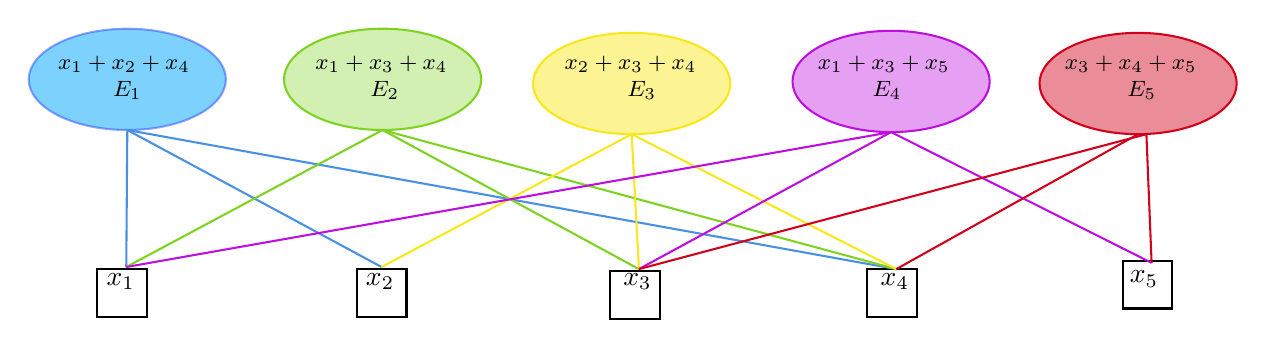
\begin{tikzpicture}[x=0.75pt,y=0.75pt,yscale=-1,xscale=1]
%uncomment if require: \path (0,300); %set diagram left start at 0, and has height of 300

%Shape: Ellipse [id:dp5233787389347726] 
\draw  [color={rgb, 255:red, 44; green, 73; blue, 253 }  ,draw opacity=0.5 ][fill={rgb, 255:red, 17; green, 172; blue, 251 }  ,fill opacity=0.55 ] (48,42.41) .. controls (48,28.93) and (69.27,18) .. (95.5,18) .. controls (121.73,18) and (143,28.93) .. (143,42.41) .. controls (143,55.89) and (121.73,66.81) .. (95.5,66.81) .. controls (69.27,66.81) and (48,55.89) .. (48,42.41) -- cycle ;
%Shape: Ellipse [id:dp39789862645481744] 
\draw  [color={rgb, 255:red, 126; green, 211; blue, 33 }  ,draw opacity=1 ][fill={rgb, 255:red, 126; green, 211; blue, 33 }  ,fill opacity=0.35 ] (171,42.41) .. controls (171,28.93) and (192.27,18) .. (218.5,18) .. controls (244.73,18) and (266,28.93) .. (266,42.41) .. controls (266,55.89) and (244.73,66.81) .. (218.5,66.81) .. controls (192.27,66.81) and (171,55.89) .. (171,42.41) -- cycle ;
%Shape: Ellipse [id:dp8505513077305478] 
\draw  [color={rgb, 255:red, 248; green, 231; blue, 28 }  ,draw opacity=1 ][fill={rgb, 255:red, 248; green, 231; blue, 28 }  ,fill opacity=0.48 ] (291,44.41) .. controls (291,30.93) and (312.27,20) .. (338.5,20) .. controls (364.73,20) and (386,30.93) .. (386,44.41) .. controls (386,57.89) and (364.73,68.81) .. (338.5,68.81) .. controls (312.27,68.81) and (291,57.89) .. (291,44.41) -- cycle ;
%Shape: Ellipse [id:dp42938864023855716] 
\draw  [color={rgb, 255:red, 189; green, 16; blue, 224 }  ,draw opacity=1 ][fill={rgb, 255:red, 189; green, 16; blue, 224 }  ,fill opacity=0.4 ] (416,43.41) .. controls (416,29.93) and (437.27,19) .. (463.5,19) .. controls (489.73,19) and (511,29.93) .. (511,43.41) .. controls (511,56.89) and (489.73,67.81) .. (463.5,67.81) .. controls (437.27,67.81) and (416,56.89) .. (416,43.41) -- cycle ;
%Shape: Ellipse [id:dp5462374015203637] 
\draw  [color={rgb, 255:red, 208; green, 2; blue, 27 }  ,draw opacity=1 ][fill={rgb, 255:red, 208; green, 2; blue, 27 }  ,fill opacity=0.45 ] (535,44.41) .. controls (535,30.93) and (556.27,20) .. (582.5,20) .. controls (608.73,20) and (630,30.93) .. (630,44.41) .. controls (630,57.89) and (608.73,68.81) .. (582.5,68.81) .. controls (556.27,68.81) and (535,57.89) .. (535,44.41) -- cycle ;
%Shape: Rectangle [id:dp39502637776877325] 
\draw   (81,133.81) -- (105,133.81) -- (105,156.81) -- (81,156.81) -- cycle ;
%Shape: Rectangle [id:dp7646530195596477] 
\draw   (206,133.81) -- (230,133.81) -- (230,156.81) -- (206,156.81) -- cycle ;
%Straight Lines [id:da5140306236752665] 
\draw [color={rgb, 255:red, 74; green, 144; blue, 226 }  ,draw opacity=1 ]   (95.5,66.81) -- (95,132.81) ;
%Straight Lines [id:da29458648798494447] 
\draw [color={rgb, 255:red, 74; green, 144; blue, 226 }  ,draw opacity=1 ]   (95.5,66.81) -- (218,132.81) ;
%Shape: Rectangle [id:dp6540796767238999] 
\draw   (328,134.81) -- (352,134.81) -- (352,157.81) -- (328,157.81) -- cycle ;
%Shape: Rectangle [id:dp819419367215283] 
\draw   (452,133.81) -- (476,133.81) -- (476,156.81) -- (452,156.81) -- cycle ;
%Shape: Rectangle [id:dp9680430250943379] 
\draw   (575,129.81) -- (599,129.81) -- (599,152.81) -- (575,152.81) -- cycle ;
%Straight Lines [id:da05256627696526639] 
\draw [color={rgb, 255:red, 74; green, 144; blue, 226 }  ,draw opacity=1 ]   (95.5,66.81) -- (466,133.81) ;
%Straight Lines [id:da23133924997521804] 
\draw [color={rgb, 255:red, 126; green, 211; blue, 33 }  ,draw opacity=1 ]   (218.5,66.81) -- (95,132.81) ;
%Straight Lines [id:da9889407004920752] 
\draw [color={rgb, 255:red, 126; green, 211; blue, 33 }  ,draw opacity=1 ]   (218.5,66.81) -- (342,133.81) ;
%Straight Lines [id:da7273538025406256] 
\draw [color={rgb, 255:red, 126; green, 211; blue, 33 }  ,draw opacity=1 ]   (218.5,66.81) -- (466,133.81) ;
%Straight Lines [id:da9082603245606358] 
\draw [color={rgb, 255:red, 248; green, 231; blue, 28 }  ,draw opacity=1 ]   (338.5,68.81) -- (218,132.81) ;
%Straight Lines [id:da07715957413725438] 
\draw [color={rgb, 255:red, 248; green, 231; blue, 28 }  ,draw opacity=1 ]   (338.5,68.81) -- (342,133.81) ;
%Straight Lines [id:da02616675166554372] 
\draw [color={rgb, 255:red, 248; green, 231; blue, 28 }  ,draw opacity=1 ]   (338.5,68.81) -- (466,133.81) ;
%Straight Lines [id:da5103865657978819] 
\draw [color={rgb, 255:red, 189; green, 16; blue, 224 }  ,draw opacity=1 ]   (463.5,67.81) -- (95,132.81) ;
%Straight Lines [id:da037677573532087116] 
\draw [color={rgb, 255:red, 189; green, 16; blue, 224 }  ,draw opacity=1 ]   (463.5,67.81) -- (342,133.81) ;
%Straight Lines [id:da7338576037484348] 
\draw [color={rgb, 255:red, 189; green, 16; blue, 224 }  ,draw opacity=1 ]   (463.5,67.81) -- (589,130.81) ;
%Straight Lines [id:da5743682087969624] 
\draw [color={rgb, 255:red, 208; green, 2; blue, 27 }  ,draw opacity=1 ]   (586.5,68.81) -- (342,133.81) ;
%Straight Lines [id:da44710187097254805] 
\draw [color={rgb, 255:red, 208; green, 2; blue, 27 }  ,draw opacity=1 ]   (582.5,68.81) -- (466,133.81) ;
%Straight Lines [id:da5976449140902116] 
\draw [color={rgb, 255:red, 208; green, 2; blue, 27 }  ,draw opacity=1 ]   (586.5,68.81) -- (589,130.81) ;

% Text Node
\draw (54,27.4) node [anchor=north west][inner sep=0.75pt]  [font=\footnotesize]  {$ \begin{array}{l}
x_{1} +x_{2} +x_{4}\\
\ \ \ \ \ \ \ {\textstyle E_1}
\end{array}$};
% Text Node
\draw (178,27.4) node [anchor=north west][inner sep=0.75pt]  [font=\footnotesize]  {$ \begin{array}{l}
x_{1} +x_{3} +x_{4}\\
\ \ \ \ \ \ \ E_2
\end{array}$};
% Text Node
\draw (298,27.4) node [anchor=north west][inner sep=0.75pt]  [font=\footnotesize]  {$ \begin{array}{l}
x_{2} +x_{3} +x_{4}\\
\ \ \ \ \ \ \ \ E_3
\end{array}$};
% Text Node
\draw (420,27.4) node [anchor=north west][inner sep=0.75pt]  [font=\footnotesize]  {$ \begin{array}{l}
x_{1} +x_{3} +x_{5}\\
\ \ \ \ \ \ \ E_4
\end{array}$};
% Text Node
\draw (539,27.4) node [anchor=north west][inner sep=0.75pt]  [font=\footnotesize]  {$ \begin{array}{l}
x_{3} +x_{4} +x_{5}\\
\ \ \ \ \ \ \ \ E_5
\end{array}$};
% Text Node
\draw (84,134.4) node [anchor=north west][inner sep=0.75pt]    {$x_{1}$};
% Text Node
\draw (333,134.4) node [anchor=north west][inner sep=0.75pt]    {$x_{3}$};
% Text Node
\draw (457,134.4) node [anchor=north west][inner sep=0.75pt]    {$x_{4}$};
% Text Node
\draw (577,133.21) node [anchor=north west][inner sep=0.75pt]    {$x_{5}$};
% Text Node
\draw (209,134.4) node [anchor=north west][inner sep=0.75pt]    {$x_{2}$};
% Text Node
\draw (455,134.4) node [anchor=north west][inner sep=0.75pt]    {$$};


\end{tikzpicture}

\end{center}
Luego tenemos que para ver que bits cumplen las ecuaciones y ver si debemos cambiar alguno realizamos el siguiente cálculo

\[
\begin{array}{|c|c|c|c|c|c|c|c|}
\hline
x & E_1=1 & E_2=0 & E_3=1 & E_4=0 & E_5=1 & \text{Ceros totales}\\
\hline
x_1= 1& 1 & 1 & - & 1 & - & 0 \\
\hline
x_2=1& 1&-& 0& - &-&1\\
\hline
x_3=0& -& 1& 0 & 1 & 0 &\textcolor{gray}{2}\\
\hline
x_4=1& 1&1&0&-&0&\textcolor{gray}{2}\\
\hline
x_5=1&-&-&-&1&0&1\\
\hline
\end{array}
\]
Teniendo en cuenta esos valores, vamos a empezar a realizar los cambios en los valores de la primera columna, puesto que suponemos que las sumas tienen el bit correcto, para facilidad de lectura cada tabla de operaciones tendra el nombre de un paso para asi poder devolvernos de manera sencilla en caso de que se presenten bucles.\\
\textbf{Paso 1:} Cambiamos el valor de $x_3$, de acuerdo con el criterio podemos elegir cualquiera entre $x_3$ y $x_4$, pero en este caso elegimos $x_3$
\[
\begin{array}{|c|c|c|c|c|c|c|c|}
\hline
x & E_1=1 & E_2=0 & E_3=1 & E_4=0 & E_5=1 & \text{Ceros totales}\\
\hline
x_1= 1& 1 & 0& - & 0& - &\textcolor{gray}{2}\\
\hline
x_2=1& 1&-& 1&- &-&0\\
\hline
\textcolor{cyan}{x_3}=1&-&0&1&0&1&\textcolor{gray}{2}\\
\hline
x_4=1& 1&0&1&-&1&1\\
\hline
x_5=1&-&-&-&0&1&1\\
\hline
\end{array}
\]
Como el criterio dice que debemos cambiar alguno de los que más presenta errores y cambiar $x_3$ es devolverse al problema inicial, entonces cambiemos $x_1$.\\
\textbf{Paso 2:} Cambiamos el valor de $x_1$ y como resultado tenemos que
\[
\begin{array}{|c|c|c|c|c|c|c|c|}
\hline
x & E_1=1 & E_2=0 & E_3=1 & E_4=0 & E_5=1 & \text{Ceros totales}\\
\hline
\textcolor{cyan}{x_1}= 0& 0 & 1& - & 1& - &\textcolor{gray}{1}\\
\hline
x_2=1& 0&-& 1&- &-&\textcolor{gray}{1}\\
\hline
x_3=1&-&1&1&1&1&0\\
\hline
x_4=1& 0&1&1&-&1&\textcolor{gray}{1}\\
\hline
x_5=1&-&-&-&1&1&0\\
\hline
\end{array}
\]
En este caso no podemos volver a cambiar el valor de $x_1$ porque estaríamos devolviendonos un paso, por lo cual vamos a elegir cambiar $x_2$, se podría hacer el cambio con $x_4$ sin embargo lo haremos en caso de ser necesario más adelante.

\textbf{Paso 3:} Cambiamos el valor de $x_2$ y realizamos los cálculos obteniendo que 
$$
\begin{array}{|c|c|c|c|c|c|c|c|}
\hline
x & E_1=1 & E_2=0 & E_3=1 & E_4=0 & E_5=1 & \text{Ceros totales}\\
\hline
x_1= 0& 1 & 1& - & 1& - &0\\
\hline
\textcolor{cyan}{x_2}=0& 1&-& 0&- &-&\textcolor{gray}{1}\\
\hline
x_3=1&-&1&0&1&1&\textcolor{gray}{1}\\
\hline
x_4=1& 1&1&0&-&1&\textcolor{gray}{1}\\
\hline
x_5=1&-&-&-&1&1&0\\
\hline
\end{array}
$$
En este caso no podemos cambiar $x_2$ porque tendiamos un paso ya estudiado (Paso 2) y por los criterios aunque podemos elegir a $x_3$ o $x_4$ vamos a elegir a $x_4$.

\textbf{Paso 4:} Cambiamos el valor de $x_4$ y calculamos 
$$
\begin{array}{|c|c|c|c|c|c|c|c|}
\hline
x & E_1=1 & E_2=0 & E_3=1 & E_4=0 & E_5=1 & \text{Ceros totales}\\
\hline
x_1= 0& 0 & 0& - & 1& - &2\\
\hline
x_2=0& 0&-& 1&- &-&1\\
\hline
x_3=1&-&0&1&1&0&2\\
\hline
\textcolor{cyan}{x_4}=0& 0&0&1&-&0&\textcolor{gray}{3}\\
\hline
x_5=1&-&-&-&1&0&1\\
\hline
\end{array}
$$
Aqui el algoritmo nos dice que tenemos que cambiar el valor de $x_4$ y eso sería devolverse al paso inmediatamente anterior, por lo cual tenemos un \textbf{bluce} para este caso.
Por lo cual retomamos las opciones que nos daba el (Paso 3), es decir cambiar el valor de $x_3$

\textbf{Paso 5:} Volvemos un paso y cambiamos $x_3$
$$
\begin{array}{|c|c|c|c|c|c|c|c|}
\hline
x & E_1=1 & E_2=0 & E_3=1 & E_4=0 & E_5=1 & \text{Ceros totales}\\
\hline
x_1= 0& 1 & 0& - & 0& - &2\\
\hline
x_2=0& 1&-& 1&- &-&0\\
\hline
\textcolor{cyan}{x_3}=0&-&0&1&0&0&\textcolor{gray}{3}\\
\hline
x_4=1& 1&0&1&-&0&2\\
\hline
x_5=1&-&-&-&0&0&2\\
\hline
\end{array}
$$
Aqui el algoritmo nos dice que tenemos que cambiar el valor de $x_3$ y eso seria devolverse al (Paso 2) por lo cual entramos en un \textbf{bucle}, al finalizar el (Paso 2) elegimos cambiar el valor de $x_2$ y eso nos llevó a un \textbf{bucle} por lo cual vamos a devolvernos y cambiar esa escogencia y vamos a cambiar $x_4$\\
\textbf{Paso 6:} Volvemos al final del paso 2 y cambiamos $x_4$
$$
\begin{array}{|c|c|c|c|c|c|c|c|}
\hline
x & E_1=1 & E_2=0 & E_3=1 & E_4=0 & E_5=1 & \text{Ceros totales}\\
\hline
x_1= 0& 1 & 0& - & 1& - &1\\
\hline
x_2=1& 1&-& 0&- &-&1\\
\hline
x_3=1&-&0&0&1&0&\textcolor{gray}{3}\\
\hline
\textcolor{cyan}{x_4}=0& 1&0&0&-&0&\textcolor{gray}{3}\\
\hline
x_5=1&-&-&-&0&0&2\\
\hline
\end{array}
$$
En este caso solo podemos cambiar el valor de $x_3$, porque como lo hemos explicado anteriormente cambiar $x_4$ seria devolvernos un paso.

\textbf{Paso 7:} Cambiamos el valor de $x_3$
$$
\begin{array}{|c|c|c|c|c|c|c|c|}
\hline
x & E_1=1 & E_2=0 & E_3=1 & E_4=0 & E_5=1 & \text{Ceros totales}\\
\hline
x_1= 0& 1 & 1& - & 0& - &\textcolor{gray}{1}\\
\hline
x_2=1& 1&-& 1&- &-&0\\
\hline
\textcolor{cyan}{x_3}=0&-&1&1&0&1&\textcolor{gray}{1}\\
\hline
x_4=0& 1&1&1&-&1&0\\
\hline
x_5=1&-&-&-&0&1&\textcolor{gray}{1}\\
\hline
\end{array}
$$
En este caso podemos hacer el cambio para el siguiente paso con $x_1$ y $x_5$ para este caso escogemos $x_1$

\textbf{Paso 8:} Cambiamos el valor de $x_1$\\
$$
\begin{array}{|c|c|c|c|c|c|c|c|}
\hline
x & E_1=1 & E_2=0 & E_3=1 & E_4=0 & E_5=1 & \text{Ceros totales}\\
\hline
\textcolor{cyan}{x_1}= 1& 0 & 0& - & 1& - &\textcolor{gray}{2}\\
\hline
x_2=1& 0&-& 1&- &-&1\\
\hline
x_3=0&-&0&1&1&1&1\\
\hline
x_4=0& 0&0&1&-&1&\textcolor{gray}{2}\\
\hline
x_5=1&-&-&-&1&1&0\\
\hline
\end{array}
$$
\textbf{Paso 9:} Cambiamos el valor de $x_4$\\

$$
\begin{array}{|c|c|c|c|c|c|c|c|}
\hline
x & E_1=1 & E_2=0 & E_3=1 & E_4=0 & E_5=1 & \text{Ceros totales}\\
\hline
x_1= 1& 1 & 1& - & 1& - &0\\
\hline
x_2=1& 1&-& 0&- &-&1\\
\hline
x_3=0&-&1&0&1&0&\textcolor{gray}{2}\\
\hline
\textcolor{cyan}{x_4}=1& 1&1&0&-&0&\textcolor{gray}{2}\\
\hline
x_5=1&-&-&-&1&0&1\\
\hline
\end{array}
$$
Si realizo el cambio por $x_3$ volvería al (Paso 1) y entraría en un \textbf{bucle} y si cambio por $x_4$ también entraría en \textbf{bucle} puesto que volveria al (Paso 8). Por lo cual me devuelvo al final del (Paso 7) y realizo el cambio a $x_5$ en lugar de a $x_1$\\


\textbf{Paso 10:} Vuelvo al final del (Paso 7) y realizo el cambio al valor de $x_5$
$$
\begin{array}{|c|c|c|c|c|c|c|c|}
\hline
x & E_1=1 & E_2=0 & E_3=1 & E_4=0 & E_5=1 & \text{Ceros totales}\\
\hline
x_1= 0& 1 & 1& - & 1& - &0\\
\hline
x_2=1& 1&-& 1&- &-&0\\
\hline
x_3=0&-&1&1&1&0&\textcolor{gray}{1}\\
\hline
x_4=0& 1&1&1&-&0&\textcolor{gray}{1}\\
\hline
\textcolor{cyan}{x_5}=0&-&-&-&1&0&\textcolor{gray}{1}\\
\hline
\end{array}
$$
Por un argumento similar a los anteriores sabemos que no podemos hacer el cambio del valor a $x_5$ y escogemos cambiar el valor de $x_3$\\
\textbf{Paso 11:} Cambio al valor de $x_3$
$$
\begin{array}{|c|c|c|c|c|c|c|c|}
\hline
x & E_1=1 & E_2=0 & E_3=1 & E_4=0 & E_5=1 & \text{Ceros totales}\\
\hline
x_1= 0& 1 & 0& - & 0& - &1\\
\hline
x_2=1& 1&-& 0&- &-&1\\
\hline
\textcolor{cyan}{x_3}=1&-&0&0&0&1&\textcolor{gray}{3}\\
\hline
x_4=0& 1&0&0&-&1&2\\
\hline
x_5=0&-&-&-&0&1&1\\
\hline
\end{array}
$$
Aqui el algoritmo nos dice que cambiemos el valor de $x_3$ pero eso seria devolvenos al paso anterior, por lo cual estamos en un \textbf{bucle}. Por lo cual nos devolvemos al final del (Paso 10) y escogemos cambiar el valor de $x_4$

\textbf{Paso 12:} Vuelvo al final del (Paso 10) y realizo el cambio al valor de $x_4$
$$
\begin{array}{|c|c|c|c|c|c|c|c|}
\hline
x & E_1=1 & E_2=0 & E_3=1 & E_4=0 & E_5=1 & \text{Ceros totales}\\
\hline
x_1= 0& 0 & 0& - & 1& - &2\\
\hline
x_2=1& 0&-& 0&- &-&2\\
\hline
x_3=0&-&0&0&1&1&2\\
\hline
\textcolor{cyan}{x_4}=1& 0&0&0&-&1&\textcolor{gray}{3}\\
\hline
x_5=0&-&-&-&1&1&0\\
\hline
\end{array}
$$
Al igual que en el el (Paso 11) entro en un \textbf{bucle} puesto que el algoritmo me da como resultado volver a cambiar el valor de $x_4$.
Por lo cual debo devolverme en pasos hasta donde hice una escogencia de la cual no he probado posibilidades y eso me lleva a la tabla inicial (Paso 0) y ahi eligiriamos cambiar el valor de $x_4$ en lugar a $x_3$ sin embargo, esto presenta el mismo caso evidenciado en el (Paso 8) por lo cual entriamos en \textbf{bucle} y por lo cual, bajo el criterio de puntución teniendo en cuenta el que más falla no podriamos resolverlo y solo seria un algoritmo que notifica el error, ahora, mirarmos ahora el caso con los que presentan solo un error y un acierto, probemos con $x_2$


\textbf{Paso 13:} Probamos cambiando a $x_2$
\[
\begin{array}{|c|c|c|c|c|c|c|c|}
\hline
x & E_1=1 & E_2=0 & E_3=1 & E_4=0 & E_5=1 & \text{Ceros totales}\\
\hline
x_1= 1& 0 & 1 & - & 1 & - & 1\\
\hline
\textcolor{cyan}{x_2}=0& 0&-& 1& - &-&1\\
\hline
x_3=0& -& 1& 1 & 1 & 0 &1\\
\hline
x_4=1& 0&1&1&-&0&\textcolor{gray}{2}\\
\hline
x_5=1&-&-&-&1&0&1\\
\hline
\end{array}
\]
Como tenemos que el $x_4$ es el que tiene mayor cantidad de errores vamos a cambiarlo.

\textbf{Paso 14:} Probamos cambiando a $x_4$
\[
\begin{array}{|c|c|c|c|c|c|c|c|}
\hline
x & E_1=1 & E_2=0 & E_3=1 & E_4=0 & E_5=1 & \text{Ceros totales}\\
\hline
x_1= 1& 1 & 0 & - & 1 & - & 1\\
\hline
x_2=0& 1&-& 0& - &-&1\\
\hline
x_3=0& -& 0& 0 & 1 & 1 &\textcolor{gray}{2}\\
\hline
\textcolor{cyan}{x_4}=0& 1&0&0&-&1&\textcolor{gray}{2}\\
\hline
x_5=1&-&-&-&1&1&0\\
\hline
\end{array}
\]
Por razones análogas ya explicadas anteriormente solo podemos elegir para cambiar a $x_3$

\textbf{Paso 15:} Probamos cambiando a $x_3$
\[
\begin{array}{|c|c|c|c|c|c|c|c|}
\hline
x & E_1=1 & E_2=0 & E_3=1 & E_4=0 & E_5=1 & \text{Ceros totales}\\
\hline
x_1= 1& 1 & 1 & - & 0 & - & 0\\
\hline
x_2=0& 1&-& 1& - &-&0\\
\hline
\textcolor{cyan}{x_3}=1& -& 1& 1 & 0 & 0 &\textcolor{gray}{2}\\
\hline
x_4=0& 1&1&1&-&0&1\\
\hline
x_5=1&-&-&-&0&0&\textcolor{gray}{2}\\
\hline
\end{array}
\]
Como $x_5$ es el que tiene más errores y no se cambió en el paso inmediatamente anterior entonces el criterio nos dice que lo cambiemos

\textbf{Paso 16:} Probamos cambiando a $x_5$
\[
\begin{array}{|c|c|c|c|c|c|c|c|}
\hline
x & E_1=1 & E_2=0 & E_3=1 & E_4=0 & E_5=1 & \text{Ceros totales}\\
\hline
x_1= 1& 1 & 1 & - & 1 & - & 0\\
\hline
x_2=0& 1&-& 1& - &-&0\\
\hline
x_3=1& -& 1& 1 & 1 & 1 &0\\
\hline
x_4=0& 1&1&1&-&1&0\\
\hline
\textcolor{cyan}{x_5}=0&-&-&-&1&1&0\\
\hline
\end{array}
\]
Con lo que tenemos que el codigo original antes de cambiar por el canal era $10100$ y por lo cual habia errores en $x_2$, $x_3$, $x_4$ y $x_5$. Y el mensaje corregido es $1010010101$












\end{sol}